\chapter{\mbox{Titre G5}} % À MODIFIER

\vspace*{-7mm}
\begin{changemargin}{-10mm}{-10mm}
%pre-001
\begin{prerequis}[Connaisances \emoji{red-heart} et compétences \emoji{diamond-suit} du cycle 3]    
   \begin{itemize}        
       \item[\emoji{red-heart}] Vocabulaire associé à ces objets et à leurs propriétés : côté, sommet, angle, hauteur.
       \columnbreak
       \item[\emoji{diamond-suit}] Reconnaître, nommer, décrire des triangles, dont les triangles particuliers (triangle rectangle, triangle isocèle, triangle équilatéral).       
   \end{itemize}
\end{prerequis}
\end{changemargin}
\vspace*{-15mm}
\begin{debat}[Vocabulaire des quadrilatères] 
   \begin{changemargin}{-15mm}{-15mm}
   Le mot {\bf quadrilatère} provient du latin : {\it quatuor}, quatre, et {\it latus}, côté. Il existe un mot équivalent d'origine grecque : {\bf tétrapleure} de {\it tèssera}, quatre, et {\it pleura}, côté ou {\bf tétragone}, de {\it gônia}, angle. \\
   Comme pour les triangles, les quadrilatères peuvent être particuliers selon qu'ils ont certaines propriétés : parmi ceux-ci, on peut trouver par exemple la famille des trapèzes, des parallélogrammes, des rectangles, des losanges, des carrés ou encore des cerfs-volant. \\
   \end{changemargin}
   \begin{center}
      {\psset{unit=0.5}
      \begin{pspicture}(-1,-0.5)(14,7.5)
         \psframe[linecolor=red](7.25,0.25)(9.75,7.5)
         \psframe[linecolor=yellow](0.5,0.5)(9.5,2.5)
         \psframe[linecolor=orange](4.25,0)(10,5)
         \psframe[linecolor=orange!50](0.25,-0.25)(10.25,5.25)
         \psframe[linecolor=red!50](0,-0.5)(10.5,7.75)
         \psframe[linecolor=blue](-0.25,-0.75)(13.75,8)
         \psset{fillstyle=solid}
         \psframe[fillcolor=yellow](8,1)(9,2) %carré
         \psframe[fillcolor=yellow!50](5,1)(7,2) %rectangle
         \pspolygon[fillcolor=yellow!25](1,1)(3,1)(3,2)(1.5,2) %trapèze rectangle
         \pspolygon[fillcolor=orange!25](1,3.5)(3.5,3.5)(2.5,4.5)(1.5,4.5) %trapèze
         \pspolygon[fillcolor=orange!50](4.5,3.5)(6.25,3.5)(6.75,4.5)(5,4.5) %parallélogramme
         \pspolygon[fillcolor=orange](7.5,4)(8.5,3.5)(9.5,4)(8.5,4.5) %losange
         \pspolygon[fillcolor=red!50](3,6.5)(3,7)(5,7.5)(4.5,6) %convexe
         \pspolygon[fillcolor=red](8,6.75)(8.5,7.25)(9,6.75)(8.5,5.5) %cerf-volant
         \pspolygon[fillcolor=cyan!50](11,1.5)(13.5,3)(13,1.5)(11.25,2.5) %croisé
         \pspolygon[fillcolor=cyan](11,5)(13,5)(12.5,7)(12,5.5) %concave
      \end{pspicture}}
   \end{center}
   \begin{changemargin}{-15mm}{-15mm}
   \begin{cadre}[B2][F4]
      \begin{center}
         \hrefVideo{https://www.youtube.com/watch?v=j_seCDgA-lU}{\bf Pourquoi \og mathématiques \fg{} ?}, site Internet {\it m@ths-et-tiques} de {\it Yvan Monka}.
      \end{center}
   \end{cadre}
   \end{changemargin}
 \end{debat}

\activites
%001
% https://www.coursdeprofs.fr/publication/P-57f99zn2/TP-Activites-decouvertes-Trigonometrie.html
\begin{changemargin}{-10mm}{-10mm}
    \begin{activite}[Découverte avec GeoGebra]
        \begin{minipage}{0.6\linewidth}
            \begin{remarque}
                L'activité peut se faire :
                \begin{itemize}
                    \item En classe entière au vidéoprojecteur.
                    \item En devoir à la maison.
                    \item En salle informatique par deux.
                    \item En salle informatique individuellement.
                \end{itemize}
            \end{remarque}
        \end{minipage}
        \begin{minipage}{0.35\linewidth}
            \begin{center}
                \includegraphics[scale=0.3]{\currentpath/images/trigoIntro.png}
            \end{center}
        \end{minipage}
        \begin{center}
            % {\Huge \href{https://www.geogebra.org/m/ed8skenp}{\emoji{link} Ouvrir l'activité Geogebra}}    
            {\Huge \hrefLien{https://www.geogebra.org/classic/ed8skenp}{Ouvrir l'activité Geogebra}}    
            
        \end{center}
        \begin{enumerate}
            \item Déplacer le point$A$. Faire une remarque.
            \par\medskip
            \pointilles\par\medskip
            \pointilles\par\medskip
            \pointilles\par\medskip
            \pointilles
            \item Compléter la phrase suivante :\\
            Les rapports des longueurs de deux côtés d'un triangle rectangle \pointilles[0.3\linewidth] de la longueur des côtés.
            \item Modifier la valeur de l'angle $\widehat{ABC}$ à l'aide du curseur. Faire une remarque.
            \par\medskip
            \pointilles\par\medskip
            \pointilles\par\medskip
            \pointilles\par\medskip
            \pointilles\par\medskip        
            \item Compléter la phrase suivante :\\
            Les rapports des longueurs de deux côtés d'un triangle rectangle \pointilles[0.3\linewidth] de la mesure de l'angle $\widehat{ABC}$.
        \end{enumerate}
    
        % \textbf{Compléter la trace écrite.}
        \clearpage
        \begin{enumerate}
            \setcounter{enumi}{4}
            \item Compléter le tableau suivant en faisant bouger le curseur. Les trois derniers angles sont à choisir librement.
            
            \begin{center}
                \begin{tabular}{|c|*{7}{@{}>{\vrule width0pt height\dimexpr.65cm-.2pt\relax depth\dimexpr.35cm-.2pt\relax\centering\arraybackslash}p{\dimexpr2cm-.4pt\relax}@{}|}}
                    \hline
                    &$\widehat{ABC}$&{\red $BC$}&{\blue $BA$}&{\color{mygreen} $CA$}&$\dfrac{BA}{BC}$&$\dfrac{CA}{BC}$&$\dfrac{CA}{BA}$ \\
                    \hline
                    {\bfseries 1}&\ang{30}&{\red\num{8.155}}&{\blue\num{7.062}}&{\color{mygreen}\num{4.077}}&\num{0.866}&\num{0.5}&\num{0.577}\\
                    \hline
                    {\bfseries 2}&\ang{45}&&&&&&\\
                    \hline
                    {\bfseries 3}&\ang{60}&&&&&&\\
                    \hline
                    {\bfseries 4}&\dots&&&&&&\\
                    \hline
                    {\bfseries 5}&\dots&&&&&&\\
                    \hline
                    {\bfseries 6}&\dots&&&&&&\\
                    \hline
                \end{tabular}
            \end{center}        
            \item Compléter le tableau suivant en reprenant les angles de la question précédente et à l'aide de la calculatrice.
            
            \begin{center}
                \begin{tabular}{|c|*{4}{@{}>{\vrule width0pt height\dimexpr.65cm-.2pt\relax depth\dimexpr.35cm-.2pt\relax\centering\arraybackslash}p{\dimexpr2cm-.4pt\relax}@{}|}}
                    \hline
                    &$\widehat{ABC}$&$\cos(\widehat{ABC})$&$\sin(\widehat{ABC})$&$\tan(\widehat{ABC})$\\
                    \hline
                    {\bfseries 1}&\ang{30}&&&\\
                    \hline
                    {\bfseries 2}&\ang{45}&&&\\
                    \hline
                    {\bfseries 3}&\ang{60}&&&\\
                    \hline
                    {\bfseries 4}&\dots&&&\\
                    \hline
                    {\bfseries 5}&\dots&&&\\
                    \hline
                    {\bfseries 6}&\dots&&&\\
                    \hline
                \end{tabular}
            \end{center}        
            \item Faire une remarque en comparant les deux tableaux.
            \par\medskip
            \pointilles\par\medskip
            \pointilles\par\medskip
            \item Écrire trois égalités entre $\cos(\widehat{ABC})$; $\sin(\widehat{ABC})$; $\tan(\widehat{ABC})$ et deux côtés du triangle, $AB$, $AC$ ou $BC$.
        \end{enumerate}
    \end{activite}
    \end{changemargin}
    

\cours
%001
\begin{changemargin}{0mm}{-15mm}
    % \opset{voperator=bottom,decimalsepsymbol={,},strikedecimalsepsymbol=\rlap{,}\rule[-1pt]{3pt}{0.4pt}}
    \section{Rappels} %%%
    \begin{remarque}
        La notation fractionnaire sert notamment à écrire le quotient des divisions "interminables" par exemple le quotient de $5\div 7$ ne peut s'écrire sous forme décimale.
    \end{remarque}
    
    \vspace*{-7mm}
    \begin{minipage}[c]{0.2\linewidth}
        \pnode(2.7,0.2em){C}{\colorbox{red!30}{NUMÉRATEUR}}\\	
        \pnode(3.1,0.2em){D}{\colorbox{blue!30}{DÉNOMINATEUR}}
    \end{minipage}
    $\dfrac{\OPoval{A}{0,1}{\colorbox{red!30}{5}}}{\OPoval{B}{0,1}{\colorbox{blue!30}{7}}}$\qquad
    \ncarc[arcangle=-15]{->}{A}{C}
    \ncarc{->}{B}{D}
    \begin{minipage}[c]{0.4\linewidth}
    se lit "cinq septièmes"\\
    C'est une écriture fractionnaire du quotient    
    \end{minipage}
    $\OPoval{G}{0,1}{\colorbox{red!30}{5}} \div \OPoval{H}{0,1}{\colorbox{blue!30}{7}}$\qquad
    \begin{minipage}[c]{0.3\linewidth}
        \pnode(0,0.2em){E}{\colorbox{red!30}{DIVIDENDE}}
        \par\vspace{2.5cm}
        \pnode(0,0.2em){F}{\colorbox{blue!30}{DIVISEUR}}
    \end{minipage}
    \ncarc[arcangle=-15]{<-}{E}{G}
    \ncarc{<-}{F}{H}
    \vspace*{-10mm}

    \begin{definition}[Nombre fraction]
        Soit $a$ et $b$ deux nombres ($b\neq0$).\\
        Le {\bf quotient} $\dfrac{a}{b}$ est le nombre qui, lorsqu'il est multiplié par $b$, donne $a$, donc  $\dfrac{a}{b}\times b = a$.\\
        Ce quotient écrit sous forme d'une fraction est le résultat d'une division : $\dfrac{a}{b} =a\div b$.
    \end{definition}

    \begin{propriete}[Quotients égaux \admise]
        Le quotient de deux nombres relatifs ne change pas lorsque l'on multiplie, ou on divise, ces deux nombres par un même nombre
        relatif non nul (différent de 0).
        $$\frac{a}{b}=\frac{a\times c}{b\times c}\qquad \text{ou} \qquad \frac{a}{b}=\frac{a\div c}{b\div c}\qquad avec \quad  (b\not=0; c\not=0)$$
    \end{propriete}
\end{changemargin}
%002
\section{Technique de développement : distributivité simple}

\begin{propriete}[\admise]
    Si $a$, $b$ et $k$ sont trois nombres (connus ou inconnus) alors$$k\times(a+b)=k\times a+k\times b$$
\end{propriete}

\begin{remarque}
    \phantom{rrr}\\
    \hfill $k\times(a-b)=k\times(a+(-b))$ \hfill ou \hfill $k\times(a-b)=k\times a+k\times (-b)$ \hfill ou\hfill $k\times(a-b)=ka-kb$
\end{remarque}

\begin{propriete}[Cas particulier de distributivité]
    {\bfseries L'opposé d'une somme algébrique} est égal à la somme des {\bfseries opposés de chacun de ses termes.}
\end{propriete}

\begin{preuve}
    L'opposé d'une somme algébrique est égale au produit de cette somme par $-1$.\\
    La distribution de $-1$ sur chacun des termes de cette somme le transformera en son opposé.
\end{preuve}
\begin{remarque}
    Ces différentes formes nous permettent de d'effectuer des calculs plus facilement.
\end{remarque}
\vspace*{-5mm}
\begin{center}
   \begin{pspicture}(0,0.6)(8,2.6)
      \psset{nodesep=2mm}
      \rput(4,1.5){\large$ka\rnode{a}+kb = k(a\rnode{b}+b)$} 
      \nccurve[angleA=90,angleB=90,linecolor=A1]{->}{a}{b}
      \rput(4,2.6){\textcolor{A1}{factoriser}}
      \rput(9,1.7){\textcolor{A1}{transformer un produit en somme}}
      \rput(9,1.3){\textcolor{A1}{(on a mis les parenthèses)}}
      \nccurve[angleA=-90,angleB=-90,linecolor=B1]{->}{b}{a}
      \rput(4,0.4){\textcolor{B1}{développer}}
      \rput(-1,1.3){\textcolor{B1}{transformer une somme en produit}}
      \rput(-1,1.7){\textcolor{B1}{(on a enlevé les parenthèses)}}
   \end{pspicture}
\end{center}
\begin{exemple*1} 
   \begin{itemize}
      \item $\Circled{57}\times28-\Circled{57}\times18 =\Circled{57}\times(28-18) =\Circled{57}\times 10 =570$. 
      \item $13\times102 =\Circled{13}\times(100+2) =\Circled{13}\times100+\Circled{13}\times2 =\num{1300}+26 = \num{1326}$. 
   \end{itemize}
   \vspace*{-10mm}
\end{exemple*1}
%003
\section{Construction du symétrique d'un point}
\begin{methode*1}[Image d'un point par rapport à une droite à la règle et l'équerre]    
    \exercice
    Construire l'image d'un point $M$ par rapport à une droite $(d)$,
    
    $M$ n'appartenant pas à la droite.
    \correction
    \begin{minipage}{0.35\linewidth}
        \begin{center}
            \begin{Geometrie}
                pair M[],I,axe[];
                axe0=u*(3,0);
                axe1-axe0=u*(-0.5,2.5);                
                trace axe0--axe1 dashed dashpattern(on6bp off3bp on1.5bp off3bp) withcolor red;
                M0-axe0=u*(-1.5,0.6);
                M1=symetrie(M0,axe0,axe1);
                I= segment(M0,M1) intersectionpoint segment(axe0,axe1);
                trace segment(M0,M1);                
                trace codeperp(axe1,I,M0,5);
                label.top(TEX("axe (d)"),axe1);
                marque_s:=0.3*marque_s;
                trace marquesegment(M0,M1);
                label.ulft(TEX("$M$"),M0);
                label.urt(TEX("$M'$"),M1);
                label.urt(TEX("$I$"),I);
                trace Codelongueur(M0,I,I,M1,3);
            \end{Geometrie}
        \end{center}
    \end{minipage}
    \begin{minipage}{0.65\linewidth}
        \begin{enumerate}
            \item Tracer la perpendiculaire à l'axe (d) passant par M.
            \item Elle coupe (d) en $I$, placer le point $I$.
            \item Reporter la distance $MI$ de l'autre côté de l'axe (d).
            \item Placer le point $M'$, symétrique de $M$
        \end{enumerate}
    \end{minipage}
    \begin{myBox}{\infoComplementsNumeriques{singulier}}
        \begin{minipage}{\linewidth}
            \hrefConstruction{http://lozano.maths.free.fr/iep_local/figures_html/scr_iep_113.html}{Avec la règle et de l'équerre}
        
            \creditInstrumentPoche
        \end{minipage}
    \end{myBox}
\end{methode*1}

\begin{methode*1}[Image d'un point par rapport à une droite à la règle et au compas]    
    \exercice
    Construire l'image d'un point $M$ par rapport à une droite $(d)$,
    
    $M$ n'appartenant pas à la droite.
    \correction
    \begin{minipage}{0.35\linewidth}
        \begin{center}
            \begin{Geometrie}
                pair I,J,M[],axe[];
                path cI,cJ;
                axe0=u*(2,0);
                axe1-axe0=u*(1,5);                
                trace axe0--axe1 dashed dashpattern(on6bp off3bp on1.5bp off3bp) withcolor red;
                J=0.2[axe0,axe1];
                I=0.8[axe0,axe1];
                M0-J=u*(1.5,0.3);
                M1=symetrie(M0,I,J);
                marque_p:="croix";
                u:=u/2;
                pointe(I,J,M0,M1);
                u:=u*2;
                cI=cercles(I,M0);
                cJ=cercles(J,M0);
                trace subpath(4.8,6.8) of cI dashed evenly;
                trace subpath(0,3.6) of cJ dashed evenly;
                label.ulft(TEX("axe (d)"),axe0);
                label.lrt(TEX("$M$"),M0);
                label.lft(TEX("$M_1$"),M1);
                label.ulft(TEX("$I$"),I);
                label.lrt(TEX("$J$"),J);
            \end{Geometrie}
        \end{center}
    \end{minipage}
    \begin{minipage}{0.65\linewidth}
        \begin{enumerate}
            \item Placer deux points, $I$ et $J$, distincts sur l’axe (d), pas trop proches.
            \item Tracer deux arcs de cercle de centres $I$ et $J$, passant par $M$.
            \item Placer le point $M_1$, symétrique de $M$, à l’intersection de ces deux arcs.
        \end{enumerate}
    \end{minipage}
    \begin{myBox}{\infoComplementsNumeriques{singulier}}
        \begin{minipage}{\linewidth}
            \hrefConstruction{http://lozano.maths.free.fr/iep_local/figures_html/scr_iep_111.html}{Avec le compas}

            \creditInstrumentPoche
        \end{minipage}
    \end{myBox}
\end{methode*1}

 

%004
\section{Tangente d'un angle aigu}
\begin{definition}
    Dans un triangle {\bfseries rectangle}, la \textbf{tangente} d'un angle aigu est égal au rapport du côté opposé  par le côté adjacent à cet angle aigu.
\end{definition}

\begin{exemples*1}
    Dans le triangle $ABC$ rectangle en $A$, on a : 
    
    \medskip
    \begin{minipage}{0.4\linewidth}
        \begin{Geometrie}[CoinHD={(5u,4.5u)}]
            u:=0.75*u;            
            pair A,B,C;
            A=u*(1.75,1.75);
            B=u*(1.75,5.25);
            C=u*(6.25,1.75);
            trace polygone(A,B,C);
            remplis codeperp(B,A,C,8)--A--cycle withcolor noir;
            trace codeperp(B,A,C,8);
            trace appelation(A,B,8mm,btex Côté opposé etex);
            trace appelation(A,B,3mm,btex à l'angle $\widehat{ACB}$ etex);
            trace appelation(A,C,-3mm,btex Côté adjacent etex);
            trace appelation(A,C,-8mm,btex à l'angle $\widehat{ACB}$etex);
            trace appelation(B,C,3mm,btex Hypoténuse etex);
            marque_a:=marque_a*1.5;    
            trace marqueangle(B,C,A,0);
            label.llft(btex A etex,A);
            label.lrt(btex C etex,C);
            label.top(btex B etex,B);
        \end{Geometrie}
    \end{minipage}
    \begin{minipage}{0.55\linewidth}        
        $$\tan\widehat{ABC}=\frac{\mbox{côté opposé à l'angle $\widehat{ABC}$}}{\mbox{côté adjacent à l'angle $\widehat{ABC}$}}=\frac{AC}{AB}$$
        $$\tan\widehat{ACB}=\frac{\mbox{côté opposé à l'angle $\widehat{ACB}$}}{\mbox{côté adjacent à l'angle $\widehat{ACB}$}}=\frac{AB}{AC}$$
    \end{minipage}
\end{exemples*1}




\exercicesbase
\begin{changemargin}{-10mm}{-10mm}
\begin{colonne*exercice}    % Décommenter pour avoir un affichage sur deux colonnes    
    %001
    \begin{exercice*}
    On considère la grille ci-dessous, où les droites qui semblent parallèles le sont.

    \Reseau[%
        Colonnes=5,%
        Lignes=8,%
        Traces={%	
            pair A,B,C,D,E,F,G,H; % Placement dans le quadrillage en calculant
            A=ppreseau(0,8);
            B=ppreseau(1,8);
            C=ppreseau(1,7);
            D=ppreseau(0,7);
            E=ppreseau(2,5);
            F=ppreseau(1,2);
            G=ppreseau(3,2);
            H=ppreseau(4,6);
            marque_p:="croix";
            drawoptions(withcolor red);
            pointe(A,B,C,D,E,F,G,H);
            label.urt(btex $A$ etex,A);
            label.urt(btex $B$ etex,B);
            label.urt(btex $C$ etex,C);
            label.urt(btex $D$ etex,D);
            label.urt(btex $E$ etex,E);
            label.urt(btex $F$ etex,F);
            label.urt(btex $G$ etex,G);
            label.urt(btex $H$ etex,H);
            drawoptions();
        }]{}
    \begin{enumerate}
        \item Justifier la nature du quadrilatère $ABCD$.
        \item Déterminer l'image de $D$ par la translation qui transforme $C$ en $B$. Justifier.
        \item Déterminer l'image de $C$ par la translation qui transforme $B$ en $A$. Justifier.
    \end{enumerate}    
\end{exercice*}
\begin{corrige}
    %\setcounter{partie}{0} % Pour s'assurer que le compteur de \partie est à zéro dans les corrigés
    % \phantom{rrr}
    On considère la grille ci-dessous, où les droites qui semblent parallèles le sont.

    \scalebox{0.7}{
    \Reseau[%
        Colonnes=5,%
        Lignes=8,%
        Traces={%	
            pair A,B,C,D,E,F,G,H; % Placement dans le quadrillage en calculant
            A=ppreseau(0,8);
            B=ppreseau(1,8);
            C=ppreseau(1,7);
            D=ppreseau(0,7);
            E=ppreseau(2,5);
            F=ppreseau(1,2);
            G=ppreseau(3,2);
            H=ppreseau(4,6);
            marque_p:="croix";
            drawoptions(withcolor red);
            pointe(A,B,C,D,E,F,G,H);
            label.urt(btex $A$ etex,A);
            label.urt(btex $B$ etex,B);
            label.urt(btex $C$ etex,C);
            label.urt(btex $D$ etex,D);
            label.urt(btex $E$ etex,E);
            label.urt(btex $F$ etex,F);
            label.urt(btex $G$ etex,G);
            label.urt(btex $H$ etex,H);
            drawoptions();
        }]{}
    }
    
    \begin{enumerate}
        \item Justifier la nature du quadrilatère $ABCD$.\\
        {\red Les côtés opposés de du quadrilatère $ABCD$ sont parallèles deux à deux donc c'est un parallélogramme.}        
        \item Déterminer l'image de $D$ par la translation qui transforme $C$ en $B$. Justifier.\\
        {\red $CBAD$ étant un parallélogramme, $A$ est l'image de $D$ par la translation qui transforme $C$ en $B$.}
        \item Déterminer l'image de $C$ par la translation qui transforme $B$ en $A$. Justifier.\\
        {\red $BADC$ étant un parallélogramme, $D$ est l'image de $C$ par la translation qui transforme $B$ en $A$.}
    \end{enumerate}
\end{corrige}


    \columnbreak
    %002
    \begin{exercice}
    Recopier et compléter les égalités suivantes.
    \begin{multicols}{2}
        \begin{spacing}{1.5}
            \begin{enumerate}
                \item $\num{4.5}+\dots =5$
                \item $\num{7.8}+\dots=8$
                \item $\num{0.8}+\dots=1$
                \item $\dots+\num{0.23}=1$
                \item $\dots+\num{5.8}=6$
                \item $\dots-\num{2.3} =2$
                \item $\dots-\num{0.9} =4$
                \item $\dots-\num{5.8} =7$
                \item $\num{7.3}-\dots =7$
                \item $8-\dots =\num{7.6}$
            \end{enumerate}
        \end{spacing}
    \end{multicols}
 \end{exercice}
 \begin{corrige}
    \begin{enumerate}
        \item $\num{4.5}+{\red \num{0.5}} =5$
        \item $\num{7.8}+{\red \num{0.2}}=8$
        \item $\num{0.8}+{\red \num{0.2}}=1$
        \item ${\red\num{0.77}}+\num{0.23}=1$
        \item ${\red\num{0.2}}+\num{5.8}=6$
        \item ${\red\num{4.3}}-\num{2.3} =2$
        \item ${\red\num{4.9}}-\num{0.9} =4$
        \item ${\red\num{12.8}}-\num{5.8} =7$
        \item $7,3-{\red\num{0.3}} =7$
        \item $8-  {\red\num{0.4}} =7,6$
    \end{enumerate}
 \end{corrige}    
    %003
    \begin{exercice*}
   Compléter le tableau pour donner le volume de chaque solide en unités de volume. Tous les empilements sont suposés pleins, mais selon les cas plusieurs vues du solide sont proposées.

   \begin{center}
   \raisebox{-0.5\totalheight}[0.5\totalheight]{\raisebox{\depth}{    
      \begin{Geometrie}[CoinBG={(-u,0)},CoinHD={(3u,3u)}]
          u:=0.4*u;
          pair A,B,C,D,E,F,G,H;
          A=u*(1,1);
          B=u*(2,1);
          F=u*(2,2);
          E=u*(1,2);
          D=A shifted (0.5u,0.4u);
          C=B shifted (0.5u,0.4u);
          H=E shifted (0.5u,0.4u);
          G=F shifted (0.5u,0.4u);
          remplis polygone(B,C,G,F) withcolor Cornsilk;
          remplis polygone(E,H,G,F) withcolor 0.7Cornsilk+0.3black;
          remplis polygone(A,B,F,E) withcolor 0.9Cornsilk+0.1black;
          trace A--B--F--E--cycle;
          trace polygone(B,C,G,F);
          trace chemin(G,H,E);
          pair O;
          O=u*(1.5,0.5);
          label(btex {\bfseries 1 unité de volume} etex,O);
      \end{Geometrie}
      }}

      {\renewcommand*{\arraystretch}{1.2}
      \begin{tabular}{|>{\centering\arraybackslash}m{0.5\linewidth}|*{4}{>{\centering\arraybackslash}m{0.1\linewidth}|}}%
          \hline
          \rowcolor{gray!20}{\bf Solide} & {\bf n°1} & {\bf n°2}  & {\bf n°3} & {\bf n°4} \\
          \hline
          {Nombre de petits cubes manquant pour former le grand cube}&$0$&&&\\
          \hline
          {Volume en unités de volume}&&&&\\
          \hline
      \end{tabular}
      }
   \end{center}
   \begin{enumerate}
      \item Solide n°1
      
         \begin{Geometrie}[CoinHD={(5u,4u)}]
            u:=0.4*u;
            pair A,B,C,D,E,F,G,H;
            A=u*(1,1);
            B=u*(2,1);
            F=u*(2,2);
            E=u*(1,2);
            pair Vx,Vy,Vz;
            Vx=u*(1,0);
            Vy=u*(0.5,0.4);
            Vz=u*(0,1);
            D=A shifted Vy;
            C=B shifted Vy;
            H=E shifted Vy;
            G=F shifted Vy;
            picture cube;
            cube = image(
               remplis polygone(B,C,G,F) withcolor Cornsilk;
               remplis polygone(E,H,G,F) withcolor 0.7Cornsilk+0.3black;
               remplis polygone(A,B,F,E) withcolor 0.9Cornsilk+0.1black;
               trace A--B--F--E--cycle;
               trace polygone(B,C,G,F);
               trace chemin(G,H,E);
            );        
            trace cube;
            for j=0 upto 2:
               for k=0 upto 2:
                  for i=0 upto 2:
                        trace cube shifted (k*Vx+(2-j)*Vy+i*Vz);
                  endfor;
               endfor;
            endfor;
         \end{Geometrie}
      \item Solide n°2
     
         \VueCubes[%
            Creation,%
            Profondeur=3,%
            Largeur=3,%
            Angle=45,%
            CouleurCube=Cornsilk]{%
               3,3,3,%
               1,3,3,%
               1,2,3%
         }

         \VueCubes[%
            Creation,%
            Profondeur=3,%
            Largeur=3,%
            Angle=-20,%
            CouleurCube=Cornsilk]{%
                  3,3,3,%
                  1,3,3,%
                  1,2,3%
         }
      \item Solide n°3
      
         \VueCubes[%
            Creation,%
            Profondeur=3,%
            Largeur=3,%
            Angle=45,%
            CouleurCube=Cornsilk]{%
                  1,2,3,%
                  1,1,2,%
                  1,2,3%
         }

         \VueCubes[%
            Creation,%
            Profondeur=3,%
            Largeur=3,%
            Angle=-20,%
            CouleurCube=Cornsilk]{%
                  1,2,3,%
                  1,1,2,%
                  1,2,3%
         }
      \item Solide n°4 : ce solide est percé de part en part, au centre de chaque face.
 
         \begin{Geometrie}
            u:=0.4*u;
            pair A,B,C,D,E,F,G,H;
            A=u*(1,1);
            B=u*(2,1);
            F=u*(2,2);
            E=u*(1,2);
            pair Vx,Vy,Vz;
            Vx=u*(1,0);
            Vy=u*(0.5,0.4);
            Vz=u*(0,1);
            D=A shifted Vy;
            C=B shifted Vy;
            H=E shifted Vy;
            G=F shifted Vy;
            picture cube;
            cube = image(
               remplis polygone(B,C,G,F) withcolor Cornsilk;
               remplis polygone(E,H,G,F) withcolor 0.7Cornsilk+0.3black;
               remplis polygone(A,B,F,E) withcolor 0.9Cornsilk+0.1black;
               trace A--B--F--E--cycle;
               trace polygone(B,C,G,F);
               trace chemin(G,H,E);
            );
            picture colonneTypeUn,colonneTypeDeux;
            colonneTypeUn = image(
            for k=0 upto 2:
               trace cube shifted (k*Vz);
            endfor;
            );
            colonneTypeDeux = image(
            trace cube;
            trace cube shifted (2*Vz);
            );
            % tranche Gauche
            trace colonneTypeUn shifted (2*Vy);
            trace colonneTypeDeux shifted (Vy);
            trace colonneTypeUn;
            % tranche Centre                
            trace colonneTypeDeux shifted (Vx+2*Vy);
            trace colonneTypeDeux shifted (Vx);
            % tranche Droite                
            trace colonneTypeUn shifted (2*Vx+2*Vy);
            trace colonneTypeDeux shifted (2*Vx+Vy);                
            trace colonneTypeUn shifted (2*Vx);                
         \end{Geometrie}
   \end{enumerate}
\end{exercice*}
\begin{corrige}
    Pas de correction
\end{corrige} 
\end{colonne*exercice}        % Décommenter pour avoir un affichage sur deux colonnes    
\pagebreak
%004
\begin{exercice*}
   Écrire chaque fraction sous la forme de la somme d'un nombre entier et d'une fraction inférieure à 1 en faisant le calcul mentalement. \medskip
   \begin{multicols}{3}
      \begin{enumerate}
         \item $\dfrac72$ \bigskip
         \item $\dfrac98$ \bigskip
         \item $\dfrac13$ \bigskip
         \item $\dfrac53$ \bigskip
         \item $\dfrac{11}{4}$ \bigskip
         \item $\dfrac{13}{4}$
      \end{enumerate}
   \end{multicols}
\end{exercice*}
%005

\begin{exercice*} %5
   Dans chaque cas, tracer une figure à main levée puis construire la figure en vraie grandeur.   
   \begin{enumerate}
      \item Un rectangle LOUP tel que : LO = \Lg[cm]{8} et LP = \Lg[cm]{6}.
      \item Un carré BLEU de côté \Lg[cm]{4}.
      \item Un rectangle NUIT tel que : UI = \Lg[cm]{9,5} et IT = \Lg[cm]{11,2}.
      \item Un carré JOUR de côté \Lg[cm]{6,2}.
   \end{enumerate}
\end{exercice*}

\end{changemargin}

% \exercicesappr
% \begin{colonne*exercice}    % Décommenter pour avoir un affichage sur deux colonnes
    \serie{\ldots}
    % %001
    % \begin{exercice*}
    Dans tout l'exercice, les points $A$, $P$ et $B$ sont alignés ainsi que les points $A$, $R$ et $C$.

    Pour chaque figure :
    \begin{itemize}
        \item Expliquer pourquoi on peut appliquer le théorème de Thalès.
        \item Écrire alors les rapports égaux.
    \end{itemize}

    \begin{enumerate}
        \item \phantom{rrr}
        
        \begin{tikzpicture}[scale=0.6]
            % \draw[help lines, color=black!30, dashed] (0,0) grid (8,12);        
            \coordinate[label=above left:$C$] (C) at (1,4);
            \coordinate[label=above left:$B$] (B) at (1,1);            
            \coordinate[label=below:$A$] (A) at (5,4);
            \tkzDefPointBy[homothety=center A ratio 0.4](C)	\tkzGetPoint{R};
            \tkzDefPointBy[homothety=center A ratio 0.4](B)	\tkzGetPoint{P};
            \tkzDefPointBy[homothety=center B ratio 1.2](C)	\tkzGetPoint{C1};
            \tkzDefPointBy[homothety=center P ratio 1.5](R)	\tkzGetPoint{R1};
            \tkzLabelPoints[above left](R);
            \tkzLabelPoints[below right](P);
            \tkzDrawLine(C,A);
            \tkzDrawLine(B,A);
            \tkzDrawLine(C,B);
            \tkzDrawLine[add=0.5 and 0.5](R,P);
            \tkzMarkRightAngle[fill=gray!20](A,R,R1);
            \tkzMarkRightAngle[fill=gray!20](A,C,C1);
        \end{tikzpicture}
        \item \phantom{rrr}
        
        \begin{tikzpicture}[scale=0.6]
            % \draw[help lines, color=black!30, dashed] (0,0) grid (8,12);        
            \coordinate[label=below left:$B$] (B) at (1,4.3);
            \coordinate[label=above:$A$] (A) at (3,4);            
            \coordinate[label=right:$C$] (C) at (1.5,3);
            \tkzDefPointBy[homothety=center A ratio -1.5](B) \tkzGetPoint{P};
            \tkzDefPointBy[homothety=center A ratio -1.5](C)	\tkzGetPoint{R};
            \tkzLabelPoints[right](R);
            \tkzLabelPoints[below left](P);
            \tkzDrawLine[add=0.5 and 0.5](B,P);
            \tkzDrawLine[add=0.5 and 0.5](C,R);
            \tkzDrawLine[add=1 and 1](B,C);
            \tkzDrawLine[add=1 and 1](R,P);
            \tkzDefPointBy[homothety=center C ratio 2](B)	\tkzGetPoint{s};
            \tkzLabelPoints[right](s);
            \tkzDefPointBy[homothety=center B ratio 1.8](C)	\tkzGetPoint{z};
            \tkzLabelPoints[right](z);
            \tkzMarkAngle[size=0.35,mark=||](P,B,s);
            \tkzDefPointBy[homothety=center P ratio 2](R)	\tkzGetPoint{t};
            \tkzLabelPoints[right](t);
            \tkzDefPointBy[homothety=center R ratio 2](P)	\tkzGetPoint{u};
            \tkzLabelPoints[left](u);
            \tkzDefPointBy[homothety=center A ratio 2](P)	\tkzGetPoint{y};
            \tkzLabelPoints[below](y);
            \tkzMarkAngle[size=0.35,mark=||](y,P,t);
            \tkzDefPointBy[homothety=center A ratio 2](B)	\tkzGetPoint{v};
            \tkzLabelPoints[above](v);
            \tkzDefPointBy[homothety=center A ratio 2](C)	\tkzGetPoint{w};
            \tkzLabelPoints[above](w);
            \tkzDefPointBy[homothety=center A ratio 1.8](R)	\tkzGetPoint{x};
            \tkzLabelPoints[below](x);
        \end{tikzpicture}

    \end{enumerate}
\end{exercice*}
\begin{corrige}
    %\setcounter{partie}{0} % Pour s'assurer que le compteur de \partie est à zéro dans les corrigés
    % \phantom{rrr}
    \begin{enumerate}
        \item Les droites $(BC)$ et $(PR)$ sont toutes les deux perpendiculaires à la droite $(AC)$.
        
        De plus les droites $(CR)$ et $(BP)$ sont sécantes en $A$.

        \medskip
        Le théorème de Thalès permet donc d'écrire $\dfrac{AR}{AC}=\dfrac{AP}{AB}=\dfrac{RP}{BC}$.

        \medskip
        \item Les droites $(BC)$ et $(PR)$ forment avec la sécante $(BP)$
        les angles  $\widehat{sBA}$ et $\widehat{RPy}$ correspondants égaux, elles sont donc parallèles.
        
        De plus les droites $(CR)$ et $(BP)$ sont sécantes en $A$.

        \medskip
        Le théorème de Thalès permet donc d'écrire $\dfrac{AB}{AP}=\dfrac{AC}{AR}=\dfrac{BC}{RP}$.

    \end{enumerate}

\end{corrige}



    \serie{\ldots}
    % %002
    % \begin{exercice*}
    Les triangles $ABC$ et $DEF$ ci-dessous sont isométriques.

    Compléter la figure sachant que $AB=DF$ 
    
    et $\widehat{ABC}=\widehat{EDF}$.

    \hspace*{-1cm}
    \begin{tikzpicture}[scale = 0.5]
        % \draw[help lines, color=gray!30, dashed] (0,0) grid (18,11);
        \coordinate[label=left:$A$] (A) at (1,4);
        \coordinate[label=above:$B$] (B) at (4,10);
        \coordinate[label=below:$C$] (C) at (4,1);        
        \draw (A) -- (B) -- (C) -- (A);
        \coordinate[label=above:$\ldots\ldots$] (E) at (8,6);
        \coordinate[label=below:$\ldots\ldots$] (F) at (11,3);
        \coordinate[label=above:$\ldots\ldots$] (D) at (17,6);
        \draw (D) -- (E) -- (F) -- (D);
        \pic [draw=black, -, angle eccentricity=1.5,angle radius=0.5cm] {angle = B--C--A};
        \pic [draw=black, -, angle eccentricity=1.5,angle radius=0.5cm] {angle = A--B--C};
        \pic [draw=black, -, angle eccentricity=1.5,angle radius=0.6cm] {angle = A--B--C};
        \pic [draw=black, -, angle eccentricity=1.5,angle radius=0.5cm] {angle = C--A--B};
        \pic [draw=black, -, angle eccentricity=1.5,angle radius=0.6cm] {angle = C--A--B};
        \pic [draw=black, -, angle eccentricity=1.5,angle radius=0.7cm] {angle = C--A--B};

        \pic [draw=black, -, angle eccentricity=1.5,angle radius=0.5cm] {angle = F--E--D};
        \pic [draw=black, -, angle eccentricity=1.5,angle radius=0.5cm] {angle = E--D--F};
        \pic [draw=black, -, angle eccentricity=1.5,angle radius=0.6cm] {angle = E--D--F};
        \pic [draw=black, -, angle eccentricity=1.5,angle radius=0.5cm] {angle = D--F--E};
        \pic [draw=black, -, angle eccentricity=1.5,angle radius=0.6cm] {angle = D--F--E};
        \pic [draw=black, -, angle eccentricity=1.5,angle radius=0.7cm] {angle = D--F--E};
    \end{tikzpicture}
\end{exercice*}
\begin{corrige}
    %\setcounter{partie}{0} % Pour s'assurer que le compteur de \partie est à zéro dans les corrigés
    \phantom{rrr}    

    \begin{tikzpicture}[scale = 0.5]
        % \draw[help lines, color=gray!30, dashed] (0,0) grid (18,11);
        \coordinate[label=left:$A$] (A) at (1,4);
        \coordinate[label=above:$B$] (B) at (4,10);
        \coordinate[label=below:$C$] (C) at (4,1);        
        \draw (A) -- (B) -- (C) -- (A);
        \coordinate[label=above:$E$] (E) at (8,6);
        \coordinate[label=below:$F$] (F) at (11,3);
        \coordinate[label=above:$D$] (D) at (17,6);
        \draw (D) -- (E) -- (F) -- (D);
        \pic [draw=black, -, angle eccentricity=1.5,angle radius=0.5cm] {angle = B--C--A};
        \pic [draw=black, -, angle eccentricity=1.5,angle radius=0.5cm] {angle = A--B--C};
        \pic [draw=black, -, angle eccentricity=1.5,angle radius=0.6cm] {angle = A--B--C};
        \pic [draw=black, -, angle eccentricity=1.5,angle radius=0.5cm] {angle = C--A--B};
        \pic [draw=black, -, angle eccentricity=1.5,angle radius=0.6cm] {angle = C--A--B};
        \pic [draw=black, -, angle eccentricity=1.5,angle radius=0.7cm] {angle = C--A--B};

        \pic [draw=black, -, angle eccentricity=1.5,angle radius=0.5cm] {angle = F--E--D};
        \pic [draw=black, -, angle eccentricity=1.5,angle radius=0.5cm] {angle = E--D--F};
        \pic [draw=black, -, angle eccentricity=1.5,angle radius=0.6cm] {angle = E--D--F};
        \pic [draw=black, -, angle eccentricity=1.5,angle radius=0.5cm] {angle = D--F--E};
        \pic [draw=black, -, angle eccentricity=1.5,angle radius=0.6cm] {angle = D--F--E};
        \pic [draw=black, -, angle eccentricity=1.5,angle radius=0.7cm] {angle = D--F--E};
    \end{tikzpicture}
\end{corrige}


    % \columnbreak
    % %003
    % \begin{exercice}[Lien avec une méthode \ExerciceRefMethode{methodeN1-exemple}]
    \label{exoN1-exemple2}
    Test pour avoir un lien avec une méthode.
\end{exercice}

    % %004
    % \begin{exercice}[Exercice sans correction][\algo]
    Exercice d'algorithmique sans correction.
\end{exercice}
  
    \serie{\ldots}
    % %005
    % \begin{exercice*}
    Pour trouver la hauteur d'une éolienne, on a les renseignements suivants :

    \begin{itemize}
        \item Les points $O$, $A$ et $C$ sont alignés.
        \item Les points $O$, $B$ et $D$ sont alignés.
        \item Les angles $\widehat{OAB}$ et $\widehat{ACD}$ sont droits.
        \item $OA = \Lg[m]{11}$.
        \item $AC = \Lg[m]{594}$.
        \item $AB = \Lg[m]{1.5}$.
    \end{itemize}

    \begin{minipage}{1\linewidth}
    \begin{center}
        La figure n'est pas à l'échelle.

        \includegraphics[scale=0.4]{\currentpath/images/eolienne.png}    
    \end{center}
    \creditLibre{Cahier iparcours 2022 de $3^e$}
    \end{minipage}    

    \begin{enumerate}
        \item Expliquer pourquoi les droites $(AB)$ et $(CD)$ sont parallèles.
        \item Calculer la hauteur $CD$ de l'éolienne. Justifier.
    \end{enumerate}
\end{exercice*}
\begin{corrige}
    %\setcounter{partie}{0} % Pour s'assurer que le compteur de \partie est à zéro dans les corrigés
    % \phantom{rrr}
    \begin{enumerate}
        \item Les droites $(AB)$ et $(CD)$ sont perpendiculaires à la même droite $(AC)$, elles sont donc parallèles entre elles.
        \item $OC = OA+AC = \Lg[m]{11}+\Lg[m]{594} = \Lg[m]{605}$
        \begin{itemize}
            \item Les droites $(BD)$ et $(AC)$ sont sécantes en $O$.
            \item $(AB)$ et $(CD)$ sont parallèles.
        \end{itemize}

        Le théorème de Thalès permet d'écrire $\dfrac{OA}{OC}=\dfrac{OB}{OD}=\dfrac{BA}{DC}$ d'où $\dfrac{11}{605}=\dfrac{OB}{OD}=\dfrac{\num{1.5}}{DC}$.

        \medskip
        D'où $CD = \dfrac{605\times \num{1.5}}{11}=\num{82.5}$.

        \medskip
        L'éolienne mesure donc \Lg{82.5}.
    \end{enumerate}
\end{corrige}




    % \pagebreak
    % %006
    % \begin{exercice*}[Cercle]
    Soit un cercle $(\mathcal{C})$ de centre $O$.

    \begin{tikzpicture}[scale = 0.5]
        % \draw[help lines, color=black!30, dashed] (0,0) grid (10,10);        
        \coordinate[label=above:$O$] (O) at (5,5);
        \draw (4.9,5)--(5.1,5);
        \draw (5,4.9)--(5,5.1);
        \draw (O) circle (4);
    \end{tikzpicture}

    % \begin{multicols}2
        \begin{enumerate}
            \item Tracer deux diamètres $[AB]$ et $[CD]$ du cercle $(\mathcal{C})$.
            \item Justifier que les trianges $AOC$ et $BOD$ sont isométriques.
            \item Faire une déduction quant aux segments $[AC]$ et $[BD]$.
            \item Déterminer la nature du quadrilatère ainsi formé.
        \end{enumerate}
    % \end{multicols}
\end{exercice*}
\begin{corrige}
    %\setcounter{partie}{0} % Pour s'assurer que le compteur de \partie est à zéro dans les corrigés
    % \begin{multicols}2
        \begin{enumerate}
            \item \phantom{rrr}
            
                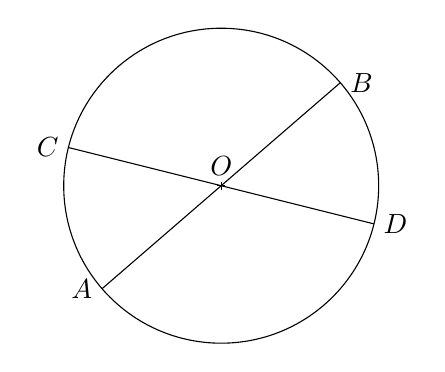
\begin{tikzpicture}[scale = 0.5]
                    % \draw[help lines, color=black!30, dashed] (0,0) grid (10,10);        
                    \coordinate[label=above:$O$] (O) at (5,5);
                    \draw (4.9,5)--(5.1,5);
                    \draw (5,4.9)--(5,5.1);
                    \draw (O) circle (4);
            
                    \coordinate[label=left:$A$] (A) at (1.97,2.38);
                    \coordinate[label=right:$B$] (B) at (8.03,7.62);
            
                    \draw (A)--(B);
            
                    \coordinate[label=left:$C$] (C) at (1.12,5.97);
                    \coordinate[label=right:$D$] (D) at (8.88,4.03);
            
                    \draw (C)--(D);
                \end{tikzpicture}

            \item Les angles $\widehat{AOC}$ et $\widehat{BOD}$ sont opposés par le sommet donc égaux.
            
            D'autre part, $OC=OD=OB=OA$ car $A$, $B$, $C$ et $D$ sont tous les quatre des points
            du cercle $(\mathcal{C})$ de centre $O$.

            Les triangles $AOC$ et $BOD$ ont un angle égal compris entre deux côtés égaux deux à deux.
            
            \psshadowbox{Ils sont donc isométriques}.
            \medskip
            \item Les triangles $AOC$ et $BOD$ sont iométriques donc $AC=BD$.
        \end{enumerate}
    % \end{multicols}
\end{corrige}


    % %007
    % \begin{exercice*}[Programme de calcul]
    Voici un programme de calcul :
    \myProgCalcul{$\leadsto$}{Programme de calcul}{%
        \ProgCalcul[Enonce,ThemePerso]{%
            Choisir un nombre.,
            Soustraire $10$ à ce nombre.,
            Multiplier le résultat par $-5$.,
            Ajouter le quintuple du nombre de départ.,
        }
    }  
    Applique ce programme à chacun de ces nombres :
    \begin{multicols}4
        \begin{enumerate}
            \item $ 3 $
            \item $ 10 $
            \item $ -2 $
            \item $ -10 $
        \end{enumerate}
    \end{multicols}
    \begin{enumerate}
        \setcounter{enumi}{4}
        \item Que remarques-tu ? Expliquer pourquoi.
    \end{enumerate}
        
\end{exercice*}
\begin{corrige}
    %\setcounter{partie}{0} % Pour s'assurer que le compteur de \partie est à zéro dans les corrigés
    \phantom{rrr}    
    \begin{multicols}2
    \begin{spacing}2
        \begin{enumerate}
            \item \ProgCalcul{3,-10 *(-5) +15}            
            \item \ProgCalcul{10,-10 *(-5) +50}            
            \item \ProgCalcul{-2,-10 *(-5) +(-10)}            
            \item \ProgCalcul{-10,-10 *(-5) +(-50)}
        \end{enumerate}
    \end{spacing}
    \end{multicols}
        \begin{enumerate}
            \setcounter{enumi}{4}
            \item On remarque que chaque fois le résultat vaut $50$. En effet :
        \end{enumerate}
        % La commande doit être en dehors de l'environnement enumerate sinon bug !
        \myProgCalcul{$\leadsto$}{Programme de calcul}{%
            \ProgCalcul[Application,SansCalcul,ThemePerso]{%                
            Soustraire $10$ à ce nombre.,
            Multiplier le résultat par $-5$.,
            Ajouter le quintuple du nombre de départ.,
            §                §
            n,-10 *(-5) +5n,n-10 -5\times(n-10)=-5n+50 -5n+50+5n=50
            }
        } 
\end{corrige}
    % %008
    % \begin{exercice*}
    On considère que ces deux tables à repasser sont posées sur un sol horizontal.

    \begin{minipage}{1\linewidth}
    \begin{center}
        La figure n'est pas à l'échelle.

        \includegraphics[scale=0.4]{\currentpath/images/tablesARepasser.png}    
    \end{center}
    \creditLibre{Cahier iparcours 2022 de $3^e$}
    \end{minipage}    

    \begin{enumerate}
        \item Déterminer si le plateau rose est horizontal?
        \item Déterminer si le plateau vert est horizontal?
    \end{enumerate}
\end{exercice*}
\begin{corrige}
    %\setcounter{partie}{0} % Pour s'assurer que le compteur de \partie est à zéro dans les corrigés
    \phantom{rrr}

    \begin{center}
        La figure n'est pas à l'échelle.

        \includegraphics[scale=0.4]{\currentpath/images/tablesARepasserCorr.png}    
    \end{center}

    \begin{enumerate}
        \item \textbf{Plateau rose}
        
        On compare les rapports $\dfrac{\num{21.6}}{52}$ et $\dfrac{25}{60}$.

        \medskip
        $\num{21.6}\times 60 = \num{1296}$ et $52\times 25 = \num{1300}$

        Les produits en croix ne sont pas égaux donc les rapports non plus.

        Si le plateau était parallèle au sol, les rapports seraient égaux d'après le 
        théorème de Thalès or ce n'est pas le cas donc le plateau rose n'est pas horizontal.
        \item \textbf{Plateau vert}

        On compare les rapports $\dfrac{18}{48}$ et $\dfrac{24}{64}$.

        \medskip
        Ces rapports sont tous les deux égaux à $\dfrac{3}{8}$

        De plus les points $A$, $E$ et $D$ d'une part et $B$, $E$ et $C$ d'autre part sont alignés dans le même ordre.

        D'après la réciproque du théorème de Thalès le plateau vert $(AB)$ est parallèle au sol $(CD)$ qui est horizontal donc le plateau vert est horizontal.

    \end{enumerate}
\end{corrige}





\end{colonne*exercice}        % Décommenter pour avoir un affichage sur deux colonnes



% REMARQUE : La commande \recreation à la place de la commande \Recreation permet de ne pas inclure un saut de page
\Recreation
\vspace*{-15mm}
%001
% Les enigmes ne sont pas numérotées par défaut donc il faut ajouter manuellement la numérotation
% si on veut mettre plusieurs enigmes
\refstepcounter{exercice}
\numeroteEnigme
\begin{enigme}
    Trouveras-tu un chemin de multiples entre les cases colorées ?

    Sans labytinthe pour tester !
\end{enigme}
  
% Pour le corrigé, il faut décrémenter le compteur, sinon il est incrémenté deux fois
\addtocounter{exercice}{-1}
\begin{corrige}
    N1 - Correction enigme de la fin de la partie cours.  

    Sans labytinthe pour tester !
\end{corrige}


% \connaissances
% % Acquis attendus en fin de chapitre
% Tableau récapitulatif des connaissances attendues en fin de chapitre
\begin{acquis}
    \titreConnaissancesAcquis{Titre commun 001}
    \begin{itemize}
    \item acquis001
    \item acquis002
    \item \ldots
    \end{itemize}
    \pagebreak
    \titreConnaissancesAcquis{Titre commun 002}
     \begin{itemize}
     \item acquis001
     \item acquis002
     \item acquis003
     \item \ldots
     \end{itemize}
\end{acquis}

\QCMautoevaluation{%
 Pour chaque question, plusieurs réponses sont proposées. Déterminer celles qui sont correctes.
}

% QCM gpe001
\begin{QCM}
    %gpe001
    \begin{EnonceCommunQCM}    
    QCM gpe 001 - Enoncé commun

    % Permet de récupérer les numéros de toutes les questions comprises entre deux marques.
    Cette consigne ne concerne que les questions \RefQCM{M1qcmgpe001Mark001} à \RefQCM{M1qcmgpe001Mark002}, \ldots
\end{EnonceCommunQCM}

    \begin{GroupeQCM}
        %gpe001exo001
        \input{\currentpath/inc/connaissancesGpre001Exo001.tex}
        %gpe001exo002
        \input{\currentpath/inc/connaissancesGpre001Exo002.tex}
        %gpe001exo003
        \begin{exercice}\label{M1qcmgpe001Mark002}
    QCM du gpe 001 concerné par la consigne commune.
    \begin{ChoixQCM}{3}
    \item proposition 001
    \item proposition 002
    \item proposition 003
    \end{ChoixQCM}
\end{exercice}
\begin{corrige}
    \reponseQCM{c}
\end{corrige}
        %gpe001exo004
        \begin{exercice*}
    QCM du gpe 001 qui n'est pas concerné par la consigne commune.
    \begin{ChoixQCM}{3}
    \item proposition 001
    \item proposition 002
    \item proposition 003
    \end{ChoixQCM}
\end{exercice*}
\begin{corrige}
    \reponseQCM{c}
\end{corrige}
    \end{GroupeQCM}
\end{QCM}

% QCM gpe002
\begin{QCM}
    %gpe002
    \begin{EnonceCommunQCM}    
    QCM gpe 002 - Enoncé commun

    % Permet de récupérer les numéros de toutes les questions comprises entre deux marques.
    Cette consigne ne concerne que les questions \RefQCM{N1qcmgpe002Mark001} à \RefQCM{N1qcmgpe002Mark002}, \ldots
\end{EnonceCommunQCM}

    \begin{GroupeQCM}
        %gpe001exo001
        \begin{exercice}\label{D1qcmgpe002Mark001}
    QCM du groupe002 concerné par la consigne ci-dessus.
    \begin{ChoixQCM}{3}
    \item proposition 001
    \item proposition 002
    \item proposition 003
    \end{ChoixQCM}
\end{exercice}
\begin{corrige}
    \reponseQCM{a}
\end{corrige}
        %gpe001exo002
        \input{\currentpath/inc/connaissancesGpre002Exo002.tex}
        %gpe001exo003
        \input{\currentpath/inc/connaissancesGpre002Exo003.tex}
        %gpe001exo004
        \input{\currentpath/inc/connaissancesGpre002Exo004.tex}
    \end{GroupeQCM}
\end{QCM}


% \TravauxPratiques
% %000
% Pas de commande \exercice ou \correction ici, ni d'environnement corrige
\begin{TP}[Titre TP Optionnel][\newLogo]
    Contenu TP
    
    Possibilité de mettre un logo perso
    \partie{Titre partie 1}
    
    TP partie 1
    
    \partie{Titre partie 2}
    
    TP partie 2
    
    \partie{Titre partie 3}
    
    TP partie 3 
\end{TP}


% % % On peut mettre un autre espace récréation après les TP par exemple mais sans corrigé possible
% \Recreation
% Après la partie TP, il n'est pas possible de proposer des correction aux énigmes de la partie récération.
%001
% Les enigmes ne sont pas numérotées par défaut donc il faut ajouter manuellement la numérotation
% si on veut mettre plusieurs enigmes
\refstepcounter{exercice}
\numeroteEnigme
\begin{enigme}
    Trouveras-tu un chemin de multiples entre les cases colorées ?

    Sans labytinthe pour tester !
\end{enigme}

% On ne peut pas utiliser l'environnement corrige après la partie TravauxPratiques



% ============================================================================================
% ======= Annexes
% ======= Interdictions a priori
% ==========> L'environnement "corrige" --> en déhors de certains envirronnements
% ==========> La commande \partie en dehors d'un exercice
%
% ======= On peut changer les couleurs des annexes avec \ChangeAnnexe{}{}{}{}
% ======= Attention il faut mettre cette commande avant le premier appel à \annexe{}
% ======= sinon ça change toutes les annexes sauf la première !
% ======= L'appel par défaut est \ChangeAnnexe{G3}{A1}{G1}{Blanc}
% ============================================================================================
% \ChangeAnnexe{J3}{H1}{J1}{Blanc}
% %001
\annexe{Titre annexe I}

\begin{cadre}[A1][A4] 
    \begin{exercice*}
        AnnexeI - Ex1
    \end{exercice*}
\end{cadre}
%002
\annexe{Titre annexe II}

\begin{cadre}[B1][B4] 
  \begin{exercice*}
    AnnexeII - Ex1
  \end{exercice*}
  \begin{exercice*}
    AnnexeII - Ex2
  \end{exercice*}
  \begin{exercice*}
    AnnexeII - Ex3
  \end{exercice*}
  \begin{exercice*}
    AnnexeII - Ex4
  \end{exercice*}
  \begin{exercice*}
    AnnexeII - Ex5
  \end{exercice*}
  \begin{exercice*}
    AnnexeII - Ex6
  \end{exercice*}
\end{cadre}

%003
\annexe{Titre annexe III}

\begin{cadre}[C1][C4] 
  \begin{exercice}
    AnnexeIII - Ex1
  \end{exercice}
\end{cadre}
